\documentclass{standalone}
\usepackage{tikz}
\usetikzlibrary{patterns, positioning}


\begin{document}
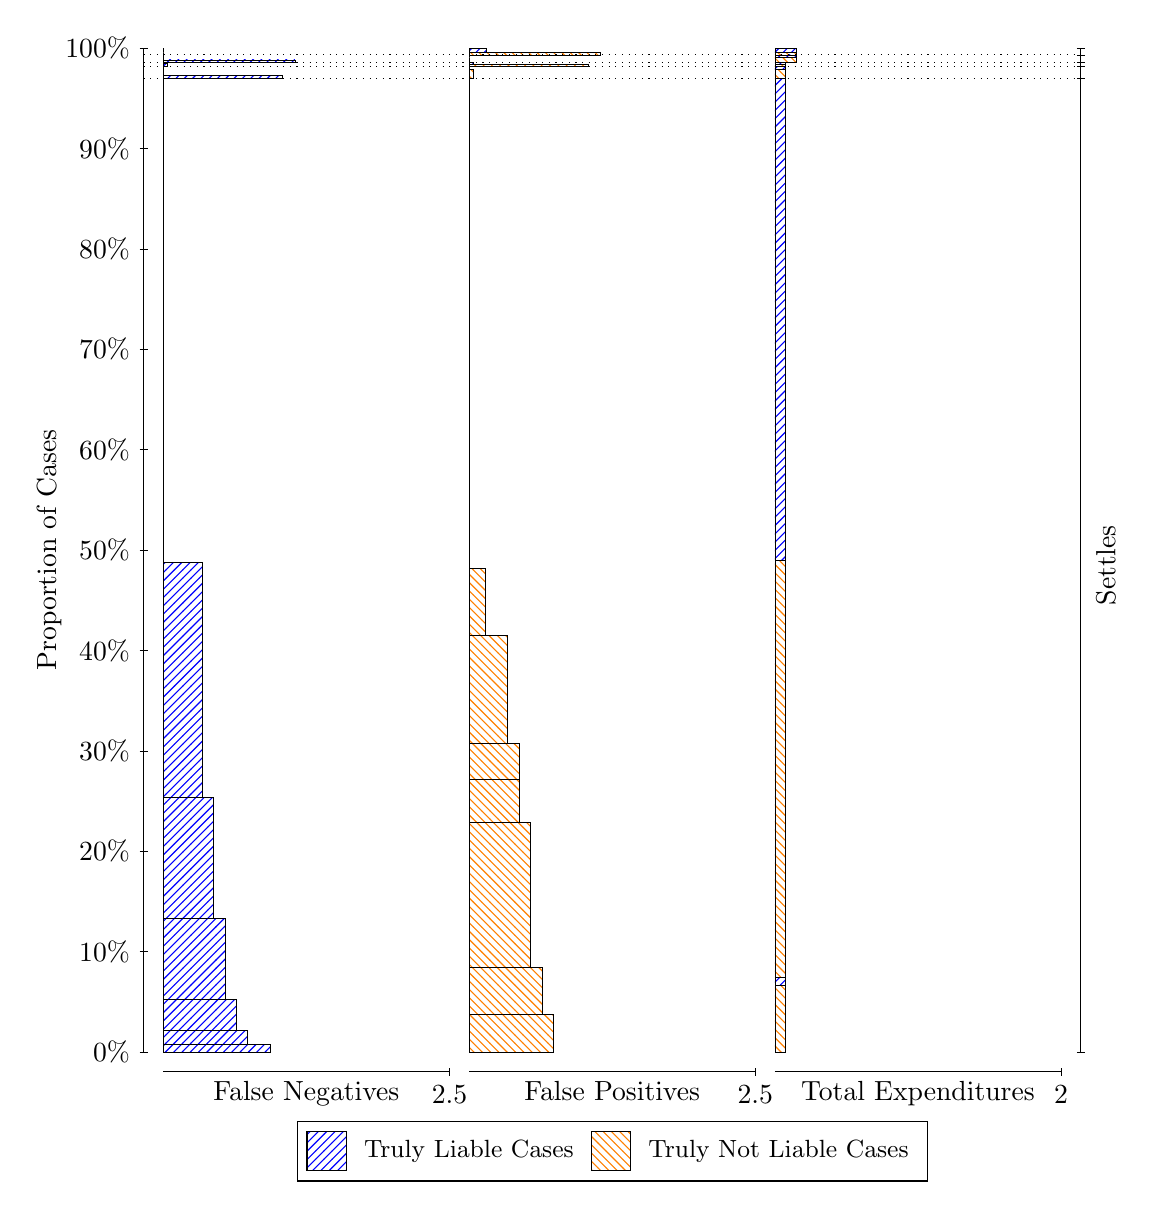
\begin{tikzpicture}
\draw[black, very thin] (1.5,1.75) -- (1.5,14.5);
\node[rotate=90, text=black, anchor=center] at (0.3, 8.125) {Proportion of Cases};
\draw[black, very thin] (1.45,1.75) -- (1.55,1.75);
\node[text=black, anchor=east] at (1.45, 1.75) {0\%};
\draw[black, very thin] (1.45,3.025) -- (1.55,3.025);
\node[text=black, anchor=east] at (1.45, 3.025) {10\%};
\draw[black, very thin] (1.45,4.3) -- (1.55,4.3);
\node[text=black, anchor=east] at (1.45, 4.3) {20\%};
\draw[black, very thin] (1.45,5.575) -- (1.55,5.575);
\node[text=black, anchor=east] at (1.45, 5.575) {30\%};
\draw[black, very thin] (1.45,6.85) -- (1.55,6.85);
\node[text=black, anchor=east] at (1.45, 6.85) {40\%};
\draw[black, very thin] (1.45,8.125) -- (1.55,8.125);
\node[text=black, anchor=east] at (1.45, 8.125) {50\%};
\draw[black, very thin] (1.45,9.4) -- (1.55,9.4);
\node[text=black, anchor=east] at (1.45, 9.4) {60\%};
\draw[black, very thin] (1.45,10.675) -- (1.55,10.675);
\node[text=black, anchor=east] at (1.45, 10.675) {70\%};
\draw[black, very thin] (1.45,11.95) -- (1.55,11.95);
\node[text=black, anchor=east] at (1.45, 11.95) {80\%};
\draw[black, very thin] (1.45,13.225) -- (1.55,13.225);
\node[text=black, anchor=east] at (1.45, 13.225) {90\%};
\draw[black, very thin] (1.45,14.5) -- (1.55,14.5);
\node[text=black, anchor=east] at (1.45, 14.5) {100\%};

\draw[black, very thin] (13.4,1.75) -- (13.4,14.5);
\draw[black, very thin] (13.35,1.75) -- (13.45,1.75);
\node[anchor=west] at (13.35, 1.75) {};
\draw[black, very thin] (13.35,14.114) -- (13.45,14.114);
\node[anchor=west] at (13.35, 14.114) {};
\draw[black, very thin] (13.35,14.27) -- (13.45,14.27);
\node[anchor=west] at (13.35, 14.27) {};
\draw[black, very thin] (13.35,14.317) -- (13.45,14.317);
\node[anchor=west] at (13.35, 14.317) {};
\draw[black, very thin] (13.35,14.413) -- (13.45,14.413);
\node[anchor=west] at (13.35, 14.413) {};
\draw[black, very thin] (13.35,14.5) -- (13.45,14.5);
\node[anchor=west] at (13.35, 14.5) {};

\draw[black, very thin, pattern color=blue, pattern=north east lines] (1.75,1.75) rectangle (3.1125,1.851);
\draw[black, very thin, pattern color=blue, pattern=north east lines] (1.75,1.851) rectangle (2.8218,2.0209);
\draw[black, very thin, pattern color=blue, pattern=north east lines] (1.75,2.0209) rectangle (2.6765,2.4151);
\draw[black, very thin, pattern color=blue, pattern=north east lines] (1.75,2.4151) rectangle (2.5312,3.4496);
\draw[black, very thin, pattern color=blue, pattern=north east lines] (1.75,3.4496) rectangle (2.3858,4.9787);
\draw[black, very thin, pattern color=blue, pattern=north east lines] (1.75,4.9787) rectangle (2.2405,7.9696);
\draw[black, very thin, pattern color=orange, pattern=north west lines] (1.75,7.9696) rectangle (1.75,14.114);
\draw[black, very thin, pattern color=blue, pattern=north east lines] (1.75,14.114) rectangle (3.2578,14.152);
\draw[black, very thin, pattern color=orange, pattern=north west lines] (1.75,14.152) rectangle (1.75,14.27);
\draw[black, very thin, pattern color=blue, pattern=north east lines] (1.75,14.27) rectangle (1.8045,14.3);
\draw[black, very thin, pattern color=orange, pattern=north west lines] (1.75,14.3) rectangle (1.75,14.317);
\draw[black, very thin, pattern color=blue, pattern=north east lines] (1.75,14.317) rectangle (3.4213,14.349);
\draw[black, very thin, pattern color=orange, pattern=north west lines] (1.75,14.349) rectangle (1.75,14.413);
\draw[black, very thin, pattern color=orange, pattern=north west lines] (1.75,14.413) rectangle (1.75,14.444);
\draw[black, very thin, pattern color=blue, pattern=north east lines] (1.75,14.444) rectangle (1.75,14.5);
\draw[black, very thin, pattern color=orange, pattern=north west lines] (5.6333,1.75) rectangle (6.7052,2.229);
\draw[black, very thin, pattern color=orange, pattern=north west lines] (5.6333,2.229) rectangle (6.5598,2.8259);
\draw[black, very thin, pattern color=orange, pattern=north west lines] (5.6333,2.8259) rectangle (6.4145,4.6667);
\draw[black, very thin, pattern color=orange, pattern=north west lines] (5.6333,4.6667) rectangle (6.2692,5.2161);
\draw[black, very thin, pattern color=orange, pattern=north west lines] (5.6333,5.2161) rectangle (6.2692,5.6679);
\draw[black, very thin, pattern color=orange, pattern=north west lines] (5.6333,5.6679) rectangle (6.1238,7.0435);
\draw[black, very thin, pattern color=orange, pattern=north west lines] (5.6333,7.0435) rectangle (5.8332,7.894);
\draw[black, very thin, pattern color=blue, pattern=north east lines] (5.6333,7.894) rectangle (5.6333,14.114);
\draw[black, very thin, pattern color=orange, pattern=north west lines] (5.6333,14.114) rectangle (5.6878,14.232);
\draw[black, very thin, pattern color=blue, pattern=north east lines] (5.6333,14.232) rectangle (5.6333,14.27);
\draw[black, very thin, pattern color=orange, pattern=north west lines] (5.6333,14.27) rectangle (7.1412,14.288);
\draw[black, very thin, pattern color=blue, pattern=north east lines] (5.6333,14.288) rectangle (5.6878,14.317);
\draw[black, very thin, pattern color=orange, pattern=north west lines] (5.6333,14.317) rectangle (5.6333,14.381);
\draw[black, very thin, pattern color=blue, pattern=north east lines] (5.6333,14.381) rectangle (5.6333,14.413);
\draw[black, very thin, pattern color=orange, pattern=north west lines] (5.6333,14.413) rectangle (7.3047,14.444);
\draw[black, very thin, pattern color=blue, pattern=north east lines] (5.6333,14.444) rectangle (5.8513,14.5);
\draw[black, very thin, pattern color=orange, pattern=north west lines] (9.5167,1.75) rectangle (9.6529,2.6005);
\draw[black, very thin, pattern color=blue, pattern=north east lines] (9.5167,2.6005) rectangle (9.6529,2.7015);
\draw[black, very thin, pattern color=orange, pattern=north west lines] (9.5167,2.7015) rectangle (9.6529,7.995);
\draw[black, very thin, pattern color=blue, pattern=north east lines] (9.5167,7.995) rectangle (9.6529,14.114);
\draw[black, very thin, pattern color=orange, pattern=north west lines] (9.5167,14.114) rectangle (9.6529,14.232);
\draw[black, very thin, pattern color=blue, pattern=north east lines] (9.5167,14.232) rectangle (9.6529,14.27);
\draw[black, very thin, pattern color=orange, pattern=north west lines] (9.5167,14.27) rectangle (9.6529,14.288);
\draw[black, very thin, pattern color=blue, pattern=north east lines] (9.5167,14.288) rectangle (9.6529,14.317);
\draw[black, very thin, pattern color=orange, pattern=north west lines] (9.5167,14.317) rectangle (9.7892,14.381);
\draw[black, very thin, pattern color=blue, pattern=north east lines] (9.5167,14.381) rectangle (9.7892,14.413);
\draw[black, very thin, pattern color=orange, pattern=north west lines] (9.5167,14.413) rectangle (9.7892,14.444);
\draw[black, very thin, pattern color=blue, pattern=north east lines] (9.5167,14.444) rectangle (9.7892,14.5);
\draw[black, dotted] (1.5,14.114) -- (13.4,14.114);
\draw[black, dotted] (1.5,14.27) -- (13.4,14.27);
\draw[black, dotted] (1.5,14.317) -- (13.4,14.317);
\draw[black, dotted] (1.5,14.413) -- (13.4,14.413);
\draw[black, very thin] (1.75,1.5) -- (5.3833,1.5);
\node[text=black, anchor=north] at (3.5667, 1.5) {False Negatives};
\draw[black, very thin] (5.3833,1.45) -- (5.3833,1.55);
\node[text=black, anchor=north] at (5.3833, 1.45) {2.5};

\draw[black, very thin] (5.6333,1.5) -- (9.2667,1.5);
\node[text=black, anchor=north] at (7.45, 1.5) {False Positives};
\draw[black, very thin] (9.2667,1.45) -- (9.2667,1.55);
\node[text=black, anchor=north] at (9.2667, 1.45) {2.5};

\draw[black, very thin] (9.5167,1.5) -- (13.15,1.5);
\node[text=black, anchor=north] at (11.333, 1.5) {Total Expenditures};
\draw[black, very thin] (13.15,1.45) -- (13.15,1.55);
\node[text=black, anchor=north] at (13.15, 1.45) {2};

\node[text=black, centered, rotate=90] at (13.72, 7.9318) {Settles};





\draw (7.449999999999999,1.5) node[draw=none] (baseCoordinate) {};
\begin{scope}[align=center]
        \matrix[scale=0.5, draw=black, below=0.5cm of baseCoordinate, nodes={draw}, column sep=0.1cm]{
            \node[rectangle, draw, minimum width=0.5cm, minimum height=0.5cm, pattern color=blue, pattern=north east lines] {}; &
            \node[draw=none, font=\small, text=black] (B) {Truly Liable Cases}; &
            \node[rectangle, draw, minimum width=0.5cm, minimum height=0.5cm, pattern color=orange, pattern=north west lines] {}; &
            \node[draw=none, font=\small, text=black] (B) {Truly Not Liable Cases}; \\
            };
\end{scope}

\end{tikzpicture}
\end{document}